%<dscrpt> Un problème sur les coniques. </dscrpt>
Dans un plan euclidien orienté muni d'un repère orthonormé $(O,\overrightarrow{i},\overrightarrow{j})$, on considère l'ellipse $E$ d'équation
\begin{displaymath}
 \frac{x^2}{a^2}+\frac{y^2}{b^2}=1
\end{displaymath}
Les foyers $F_1$ et $F_2$ ont respectivement pour coordonnées $(c,0)$, $(-c,0)$. Les sommets $A_1$ et $A_2$ ont respectivement pour coordonnées $(a,0)$, $(-a,0)$. \newline
Pour tout $d\in]-a,a[$, la droite d'équation $x=d$ coupe $E$ en deux points $M_1$ (d'ordonnée positive) et $M_2$ (d'ordonnée négative).
\begin{figure}[h!t]
   \centering
   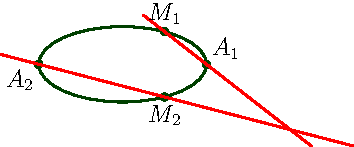
\includegraphics{Eellipse1_1.pdf}
   \caption{Droites $A_1M_1$ et $A_2M_2$.}
   \label{fig:Eellipse1_1}
\end{figure}

\begin{enumerate}
\item \begin{enumerate}
   \item Former les équations des droites $(A_1,M_1)$ et $(A_2,M_2)$.\newline
 Pour quels $d$ dans $]-a,a[$ ces droites se coupent-elles? Calculer en fonction de $d$ les coordonnées du point d'intersection lorsqu'il existe. 
   \item Former l'équation cartésienne de l'ensemble de ces points d'intersection. Quelle est cette courbe ? La dessiner en précisant le sens de parcours quand $d$ décrit $]-a,a[$ de $-a$ vers $a$.
      \end{enumerate}

\begin{figure}[h!t]
   \centering
   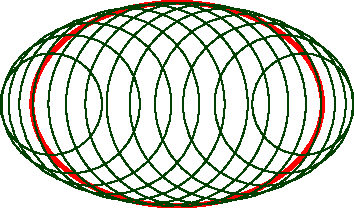
\includegraphics{Eellipse1_2.pdf}
   \caption{Quelques cercles $\Gamma_d$.}
   \label{fig:Ellipse1_2}
\end{figure}
\item Pour $d$ dans $]-a,a[$, on note $\Gamma_d$ le cercle de diamètre $M_1M_2$.
 \begin{enumerate}
\item {\'E}crire l'équation de $\Gamma_d$.
\item Soit $M_0$ un point de coordonnées $(x_0,y_0)$. Discuter suivant la position de $M_0$ dans le plan du nombre de cercles $\Gamma_d$ passant par  $M_0$.
\end{enumerate}

\begin{figure}[h!t]
   \centering
   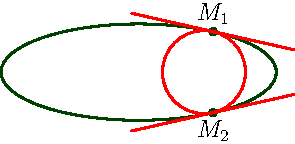
\includegraphics{Eellipse1_3.pdf}
   \caption{Cercle $C_d$.}
   \label{fig:Ellipse1_3}
\end{figure}
\item Pour $d$ dans $]-a,a[$, soit $C_d$ le cercle tangent à l'ellipse en $M_1$ et $M_2$. En ces points, le cercle et l'ellipse ont le même tangente (fig: \ref{fig:Ellipse1_3}).
\begin{enumerate}
\item Déterminer les coordonnées de son centre $\omega$.
\item Montrer que son rayon vérifie
\[r^2=-\frac{b^2}{c^2} \,(\overrightarrow{\omega F_1} / \overrightarrow{\omega F_2}) \]
\end{enumerate}
\begin{figure}[h!t]
   \centering
   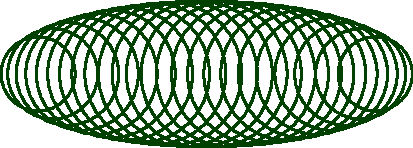
\includegraphics{Eellipse1_4.pdf}
   \caption{Quelques cercles $C_d$. Cas 1.}
   \label{fig:Ellipse1_4}
\end{figure}
\begin{figure}[h!t]
   \centering
   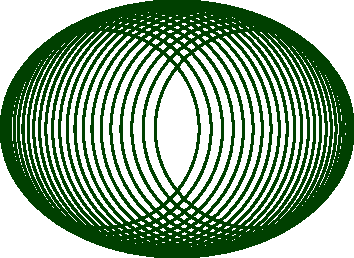
\includegraphics{Eellipse1_5.pdf}
   \caption{Quelques cercles $C_d$. Cas 2.}
   \label{fig:Ellipse1_5}
\end{figure}

\item Dans cette question, on cherche à discuter du nombre de cercles $C_d$ passant par un point $M_0$ fixé de coordonnées $x_0$ et $y_0$. On note
\begin{displaymath}
 f_{M_0}(d) = d^2-2x_0d+\frac{a^2}{c^2}(x_0^2+y_0^2-b^2)
\end{displaymath}
\begin{enumerate}
\item Montrer que $M_0 \in C_d$ si et seulement si $f_{M_0}(d) = 0$.
\item Montrer que les points $M_0$ par lesquels passe au moins un cercle $C_d$ sont dans le disque elliptique c'est à dire la portion de plan délimitée par l'ellipse $E$.
\item Exprimer, en fonction de $a$ et $b$, des réels $u$ et $v$ tels que
\begin{displaymath}
 f_{M_0}(a) = \frac{a^2}{c^2}\left( (x_0-u)^2+y_0^2-v\right) 
\end{displaymath}

\item Montrer que par $M_0$  passent  deux cercles $C_{d_1}$ et $C_{d_2}$ distincts si et seulement si $M_0$ est à dans le disque elliptique et à l'extérieur de deux disques tangents en $A_1$ et $A_2$ que l'on déterminera.
\item En distinguant deux configurations (figures \ref{fig:Ellipse1_4} et \ref{fig:Ellipse1_5}) suivant une condition à préciser liant $a$ et $b$, discuter du nombre de cercles passant par un point $M_0$.
\end{enumerate}

\item Déterminer l'ensemble des points $M_0$ tels que la tangente en $M_0$ à l'un des cercles $C_d$ passant par $M_0$ soit parallèle à $A_1A_2$.
\end{enumerate}
